\documentclass[tikz,dvipdfmx,dvipsnames]{standalone}

\usepackage{amsmath}
\usepackage{color}
\usepackage{bm}
\usepackage{mathtools}
\usepackage{physics}

\newcommand{\red}[1]{\textcolor{red}{#1}}
\newcommand{\blue}[1]{\textcolor{blue}{#1}}
\newcommand{\cyan}[1]{\textcolor{cyan}{#1}}
\newcommand{\gray}[1]{\textcolor{gray}{#1}}
\newcommand{\green}[1]{\textcolor{green}{#1}}
\newcommand{\brown}[1]{\textcolor{brown}{#1}}
\newcommand{\black}[1]{\textcolor{black}{#1}}
\newcommand{\Img}[1]{\mathrm{Im}\qty(#1)}
\newcommand{\Ker}[1]{\mathrm{Ker}\qty(#1)}
\newcommand{\Supp}[1]{\mathrm{supp}\qty(#1)}
\newcommand{\Rank}[1]{\mathrm{rank}\qty(#1)}
\newcommand{\floor}[1]{\left\lfloor #1 \right\rfloor}
\newcommand{\ceil}[1]{\left\lceil #1 \right\rceil}
% C++ (https://tex.stackexchange.com/questions/4302/prettiest-way-to-typeset-c-cplusplus)
\newcommand{\Cpp}{C\nolinebreak[4]\hspace{-.05em}\raisebox{.4ex}{\relsize{-3}{\textbf{++}}}}
% https://tex.stackexchange.com/questions/28836/typesetting-the-define-equals-symbol
\newcommand{\defeq}{\coloneqq}
\newcommand{\eqdef}{\eqqcolon}
% https://tex.stackexchange.com/questions/5502/how-to-get-a-mid-binary-relation-that-grows
\newcommand{\relmiddle}[1]{\mathrel{}\middle#1\mathrel{}}

\usetikzlibrary{
  3d,
  calc,
  math,
  matrix,
  patterns,
  backgrounds,
  arrows.meta,
  shapes.geometric
}

\definecolor{cC}{HTML}{77AC30}
\definecolor{cD}{HTML}{D95319}

\begin{document}
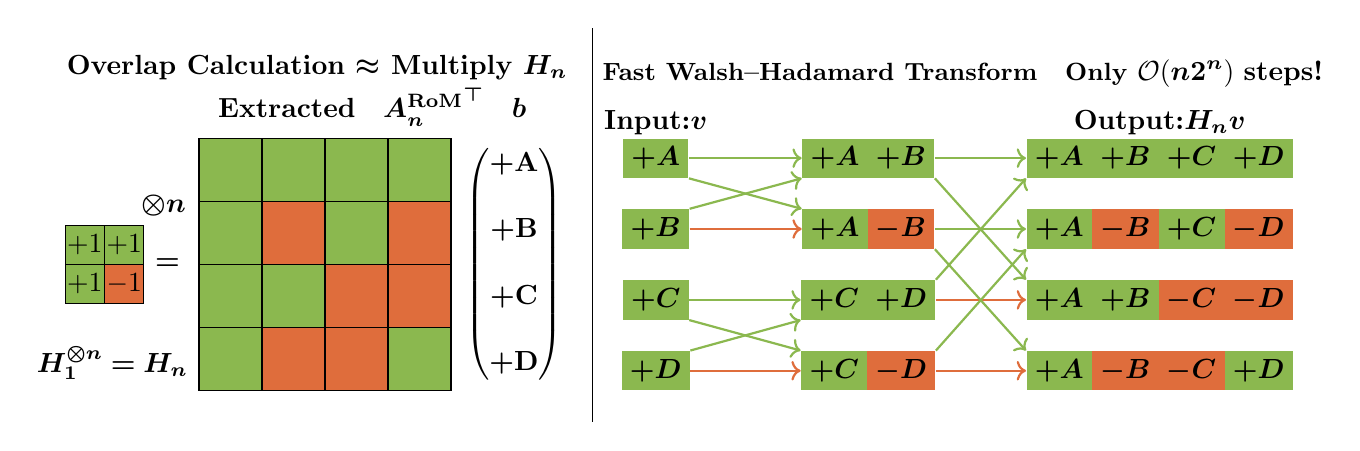
\begin{tikzpicture}
    % Define distance between nodes
    \def\dist{0.9}

    \begin{scope}
        % Define distance between nodes
        \node[align=center] at (1.5, +2.5) {\textbf{Overlap Calculation $\bm{\approx}$ Multiply $\bm{H_n}$}};
        \node[align=center] at (2.2, +2.0) {\textbf{Extracted}\quad$\bm{{A_n^{\mathrm{RoM}}}^\top}$\quad$\bm{b}$};
        \foreach \x/\y/\c in {
                0/0/cC!85!white,
                1/0/cC!85!white,
                2/0/cC!85!white,
                3/0/cC!85!white,
                0/1/cC!85!white,
                1/1/cD!85!white,
                2/1/cC!85!white,
                3/1/cD!85!white,
                0/2/cC!85!white,
                1/2/cC!85!white,
                2/2/cD!85!white,
                3/2/cD!85!white,
                0/3/cC!85!white,
                1/3/cD!85!white,
                2/3/cD!85!white,
                3/3/cC!85!white} {
                \draw[fill=\c] (0.8*\x, 1.6-0.8*\y) rectangle ({0.8*(\x+1)}, {1.6-0.8*(\y+1)});
            }

        \node at (4,0){
            $\begin{pmatrix}
                    \textbf{+A} \\[1.2em]
                    \textbf{+B} \\[1.2em]
                    \textbf{+C} \\[1.2em]
                    \textbf{+D}
                \end{pmatrix}$
        };

        \foreach \x/\y/\v/\c in {
                0/0/+1/cC!85!white,
                1/0/+1/cC!85!white,
                0/1/-1/cD!85!white,
                1/1/+1/cC!85!white} {
                \draw[fill=\c] (-0.7-0.5*\x, 0.5-0.5*\y) rectangle ({-0.7-0.5*(\x+1)}, {0.5-0.5*(\y+1)});
                \node at (-0.95-0.5*\x,0.25-0.5*\y) {$\v$};
            }
        \node at (-0.45,0.75) {$\bm{\otimes n}$};
        \node at (-0.4,0) {$\bm{=}$};
        \node at (-1.1,-1.25) {$\bm{H_1^{\otimes n}=H_n}$};

    \end{scope}

    \draw (5, -2) -- (5, 3);

    \begin{scope}[xshift=5.5cm]
        \def\xLeft{0.3}
        \def\xRight{6.7}
        \node[align=center] at (4.2, +2.7*\dist) {\textbf{\small{Fast Walsh--Hadamard Transform} \; Only} $\order{\bm{n2^n}}$ \textbf{steps!}};
        \node[align=center] at (\xLeft, +2.0*\dist) {\textbf{Input:$\bm{v}$}};
        \node[align=center] at (\xRight, +2.0*\dist) {\textbf{Output:$\bm{H_n v}$}};

        % Define coordinates for input nodes
        \node[inner sep=0pt] (A) at (\xLeft, +1.5*\dist) {\colorbox{cC!85!white}{$\bm{+A}$}};
        \node[inner sep=0pt] (B) at (\xLeft, +0.5*\dist) {\colorbox{cC!85!white}{$\bm{+B}$}};
        \node[inner sep=0pt] (C) at (\xLeft, -0.5*\dist) {\colorbox{cC!85!white}{$\bm{+C}$}};
        \node[inner sep=0pt] (D) at (\xLeft, -1.5*\dist) {\colorbox{cC!85!white}{$\bm{+D}$}};

        % Define coordinates for intermediate sum nodes
        \node[inner sep=0pt] (AB) at  (3, +1.5*\dist) {\colorbox{cC!85!white}{$\bm{+A}$}\colorbox{cC!85!white}{$\bm{+B}$}};
        \node[inner sep=0pt] (AmB) at (3, +0.5*\dist) {\colorbox{cC!85!white}{$\bm{+A}$}\colorbox{cD!85!white}{$\bm{-B}$}};
        \node[inner sep=0pt] (cD) at  (3, -0.5*\dist) {\colorbox{cC!85!white}{$\bm{+C}$}\colorbox{cC!85!white}{$\bm{+D}$}};
        \node[inner sep=0pt] (CmD) at (3, -1.5*\dist) {\colorbox{cC!85!white}{$\bm{+C}$}\colorbox{cD!85!white}{$\bm{-D}$}};

        % Define coordinates for output nodes
        \node[inner sep=0pt] (ABcD) at   (\xRight, +1.5*\dist) {\colorbox{cC!85!white}{$\bm{+A}$}\colorbox{cC!85!white}{$\bm{+B}$}\colorbox{cC!85!white}{$\bm{+C}$}\colorbox{cC!85!white}{\bm{$+D$}}};
        \node[inner sep=0pt] (AmBCmD) at (\xRight, +0.5*\dist) {\colorbox{cC!85!white}{$\bm{+A}$}\colorbox{cD!85!white}{$\bm{-B}$}\colorbox{cC!85!white}{$\bm{+C}$}\colorbox{cD!85!white}{\bm{$-D$}}};
        \node[inner sep=0pt] (ABmcD) at  (\xRight, -0.5*\dist) {\colorbox{cC!85!white}{$\bm{+A}$}\colorbox{cC!85!white}{$\bm{+B}$}\colorbox{cD!85!white}{$\bm{-C}$}\colorbox{cD!85!white}{\bm{$-D$}}};
        \node[inner sep=0pt] (AmBcD) at  (\xRight, -1.5*\dist) {\colorbox{cC!85!white}{$\bm{+A}$}\colorbox{cD!85!white}{$\bm{-B}$}\colorbox{cD!85!white}{$\bm{-C}$}\colorbox{cC!85!white}{\bm{$+D$}}};

        % Draw lines connecting the nodes
        \draw[->,thick,cC!85!white] (A) -- (AB);
        \draw[->,thick,cC!85!white] (A.south east) -- (AmB.north west);
        \draw[->,thick,cC!85!white] (B.north east) -- (AB.south west);
        \draw[->,thick,cD!85!white] (B) -- (AmB);
        \draw[->,thick,cC!85!white] (C) -- (cD);
        \draw[->,thick,cC!85!white] (C.south east) -- (CmD.north west);
        \draw[->,thick,cC!85!white] (D.north east) -- (cD.south west);
        \draw[->,thick,cD!85!white] (D) -- (CmD);
        \draw[->,thick,cC!85!white] (AB) -- (ABcD);
        \draw[->,thick,cC!85!white] (AB.south east) -- (ABmcD.north west);
        \draw[->,thick,cC!85!white] (cD.north east) -- (ABcD.south west);
        \draw[->,thick,cD!85!white] (cD) -- (ABmcD);
        \draw[->,thick,cC!85!white] (AmB) -- (AmBCmD);
        \draw[->,thick,cC!85!white] (AmB.south east) -- (AmBcD.north west);
        \draw[->,thick,cC!85!white] (CmD.north east) -- (AmBCmD.south west);
        \draw[->,thick,cD!85!white] (CmD) -- (AmBcD);
    \end{scope}
\end{tikzpicture}
\end{document}
